\chapter{Conclusiones}
\label{chap:results}

%\section{Resultados y Ejemplares obtenidos}

%\todo{Hacer}

%\section{Posibles usos y aplicaciones}

%\todo{Hacer}

%\todo{QUÉ TÍTULO LE PONEMOS A ESTO?}
\todo{Re-redactar, anda muy verde digo amarillo}

\begin{itemize}
	
	\item idea inicial
	\item Necesidad de comprender bien la sinestesia
	\item Las posibles soluciones a los problemas de análisis y composición
	\item Posibles escenarios y usos de la aplicación

\end{itemize}

El objetivo inicial del proyecto era, como se ha detallado a lo largo del documento, construir una herramienta capaz de transmitir musicalmente lo que se percibe de una imagen. Tras 9 meses de proceso de desarrollo, se puede afirmar que se ha desarrollado de forma satisfactoria una aplicación capaz de llevar a cabo dicho objetivo, así como el resto de requisitos (tanto funcionales como no funcionales) mostrados en la Sección~\ref{sec:requisitos}. Este proceso ha sido llevado a cabo por los 3 miembros del proyecto trabajando a tiempo parcial, y su resultado se puede ver en la dirección de descarga del proyecto:\\

\begin{center}
http://code.google.com/p/muphic/downloads/list
\end{center}


Para llevar a cabo la aplicación, ésta se ha dividido en dos módulos independientes que trabajan de forma secuencial: el módulo de análisis de imagen en primer lugar, y el módulo encargado de la composición musical en segundo; los cuales se pueden asemejar a la etapa de estimulación visual y a la etapa de estimulación auditiva, respectivamente. Esta distinción ha dado la posibilidad de estudiar y probar las difernetes etapas de forma independiente para poder experimentar las diferentes formas de abordar la interpretación música-imagen. Cabe destacar que, dado que esta relación debe ser objetiva y no dependiente de consideraciones culturales o personales (por especificación del sistema), se ha elegido la sinestesia como método de asociación entre la percepción visual y la auditiva.\\


Por un lado, el módulo de análisis ha resultado ser capaz de transformar cualquier tipo de imagen de entrada en una representación propia del sistema de forma suficientemente fiel en cuestión de segundos, dada una correcta configuración de parámetros por parte del usuario (las imágenes de grandes dimensiones pueden ser tratadas con menos nivel de detalle para aumentar su velocidad, por poner un ejemplo). Además, se puede cambiar la forma de reconocer formas alternando entre los distintos algoritmos de composición, permitiendo al usuario experimentar con la forma en la que quiere que una imagen sea percibida. La correcta elaboración de este módulo ha sido una pieza clave para el desarrollo del proyecto ya que, aunque sea el objetivo principal del mismo, proporciona la entrada al módulo de composición y es la pieza clave para el perfecto funcionamiento de la generación de música.\\

Por otro lado, el módulo de composición ha cumplido con las expectativas mencionadas a lo largo del documento, siendo capaz de componer melodías completamente originales que, si bien no buscan propiedades tales como ser ``pegadizas'' o musicalmente ricas, en ningún momento son disonantes. Además, el módulo permite al usuario cambiar la forma de componer cada vez, así como los instrumentos con los que sonará cada una de ellas.\\

Con todo esto, la aplicación satisface la posibilidad de ser testeada por personas sinestésiscas, de forma que éstas sean capaces de reconocer parcial o totalmente la similitud entre la imagen de entrada y la música generada. Con las diversas pruebas realizadas durante el desarrollo del proyecto, se ha determinado que la posibilidad de identificar la música creada a partir de las imágenes es factible, pero razonablemente limitada. Esto es debido a la cantidad de información que proporciona una imagen, ya que sólo en las imágenes simples (con poca información) se puede anticipar la música generada.\\


\section{Usos de la aplicación}
\label{sec:usos}

Esta aplicación ha sido desarrollada teniendo en cuenta varios tipos de mercados y no sólo los pertenecientes al sector musical, ya que además de ellos se proponen otras alternativas. Es por ello que los usos para los cuales este sistema ha sido diseñado son:

\begin{itemize} 

\item\textbf{Ayuda a la composición:} Uno de los mayores problemas a la hora de componer es la búsqueda de inspiración para crear nuevas piezas musicales. Es por ello que un generador de música de esta índole, capaz de generar piezas originales y de un estilo razonablemente predecible (ya que depende de forma determinista de una imagen de entrada) es de gran utilidad en  este ámbito, siendo capaz de proporcionar ideas a los usuarios compositores. Con el objetivo de enfocar la aplicación a este aspecto, se ha establecido contacto con varios músicos, quienes han mostrado su interés en el uso de esta aplicación para tal fin.

\item\textbf{Composición visual:} En una rama puramente artística, la asociación de imagen-música proporcionada por esta aplicación puede servir como punto de partida de obras artísticas en distintos medios elaboradas expresamente para ser interpretadas como música.

\item\textbf{Generación de música ambiente temática:} Como se ha establecido en la introducción de este documento, la generación musical desarrollada no pretende componer melodías que sean capaz de ser el foco de atención del usuario durante una gran cantidad de tiempo, sino que es su objetivo generar una música de ambiente capaz de sonar de fondo mientras el usuario realiza otra actividad. Dado que se une la percepción visual con la musical, es una forma más de realidad aumentada que puede servir como hilo musical de fondo en museos (con melodías asociadas a cuadros), anuncios (melodías asociadas al logo de la marca promocionada) o distintas estancias.

\item\textbf{Educación:} Tanto los niños pequeños como los discapacitados (con enfermedades como el autismo o similares) sienten una gran conexión con la música y están bastante atraídos por ella. Mediante el uso de esta aplicación pueden aprender a crear música de forma sencilla y además divertida, al mismo tiempo que entrena sus percepción visual, desarrollando por tanto los dos sentidos al mismo tiempo y favoreciendo su educación. Se ha comentado esta idea a personas dentro del sector educativo que han mostrado su deseo de probar esta aplicación en los cursos con alumnos más pequeños.

\end{itemize}

\section{Futuras ampliaciones}
\label{sec:ampliaciones}

Una vez desarrollada la aplicación, y siendo ésta completamente funcional, cabe plantearse las posibles ampliaciones que se podrían realizar sobre el sistema para ampliar su funcionalidad y usos. Muchas de ellas parten del idea inicial del proyecto, con la intención de robustecer el sistema o potenciar su funcionalidad; otras buscan dar al sistema un nuevo enfoque de uso. Estas ampliaciones son:

\begin{itemize}

\item\textbf{Realización de nuevos y distintos algoritmos de composición:} Aunque los algoritmos desarrollados se basan todos en una idea común (la sinestesia), existen muchas maneras de interpretar una imagen estática como una melodía que evoluciona en el tiempo. El proceso de desarrollo de estos algoritmos se basa intrínsecamente en el ensayo y error, por lo que no existe una solución definitiva. Es por esta razón que el proyecto ha sido diseñado para poder añadir nuevos algoritmos al código fuente de forma cómoda y sencilla.\\

Para ello, se puede partir de ayuda externa para producir ideas(o bien búsqueda y lectura de investigaciones llevadas a cabo sobre estos aspectos de la composición, o bien contacto con compositores profesionales). Además, es necesaria en la elaboración de nuevos algoritmos un post-proceso de testeo de la cualidad de los mismos, ya que la calidad de las piezas musicales generadas por un algoritmo no se puede demostrar con completa seguridad hasta la finalización de la implementación de los algoritmos.

\item\textbf{Permitir la inclusión de nuevos algoritmos externos en el código fuente.} Actualmente, la única manera de incluir nuevos algoritmos de composición o análisis es incluyéndolos al código fuente de la aplicación. Una posible vía de desarrollo consistiría en dar la oportunidad al usuario de incluir nuevas formas de componer y analizar de forma externa, mediante nuevos módulos ejecutables o scripts que la aplicación sea capaz de lanzar; siempre y cuando estos cumplan la especificación de los módulos de análisis/composición.\\

\item\textbf{Expandir el formato de representación de imágenes}, de forma que sea capaz de almacenar más información sobre la imagen. La aplicación desarrollada sólo es capaz de representar internamente polígonos y sus posiciones y colores; pero hay mucha más información dentro de una imagen que nos puede ser útil:

	\begin{itemize}
	
		\item\textit{Reconocimiento de simetrías:} una imagen puede diferentes tipos de simetrías entre los objetos/colores que la forman. Información de este tipo puede servir de base a nuevos algoritmos de composición para que realicen melodías que repitan patrones o segmentos en función de las simetrías encontradas.
		
		\item\textit{Reconocimiento de composiciones:} no es poco común que las figuras de una imagen estén dispuestas siguiendo formas geométricas básicas (círculos o triángulos, por poner dos ejemplos). Un ejemplo bastante famoso se puede observar en la Figura~\ref{fig:composition}, donde se muestra la imagen de entrada a la izquierda y la composición que se pretende reconocer a la derecha. Imágenes con composiciones muy marcadas pueden producir melodías en las que las melodías de las figuras dentro de una misma composición estén muy relacionadas.\\
			
			\begin{figure}[!htbp]
			\centering
			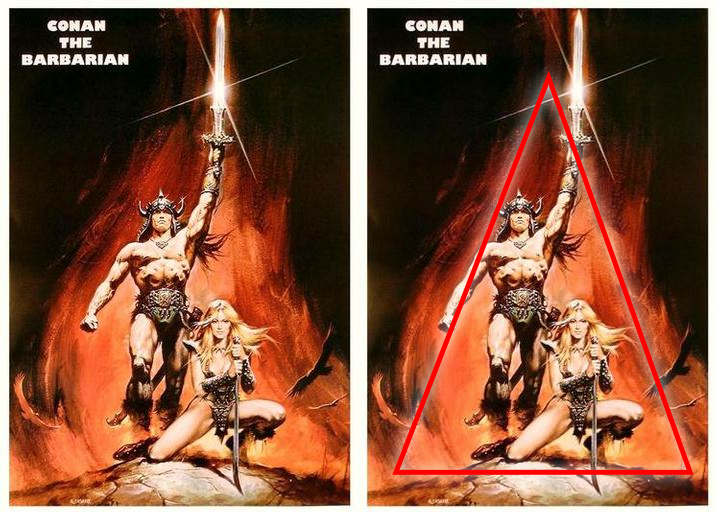
\includegraphics[scale=0.47]{graphics/composition2.png}
			\caption{Ejemplo de reconocimiento de una composición triangular.}
			\label{fig:composition}
			\end{figure}
		
		\item\textit{Reconocimiento de estructuras fractales:} de forma más ambiciosa, el proceso de análisis podría distinguir aquellos casos en los que las figuras de una imagen forman entre sí estructuras fractales, es decir, donde formas básicas se repiten en diferentes dimensiones, como se da en la figura. Esta característica es bastante útil, ya que existen numerosos estudios en el campo de la composición algorítmica basados en estructuras fractales; se podría hacer uso de dichas investigaciones si se consiguiera reconocer esta característica.
		
			\begin{figure}[!htbp]
			\centering
			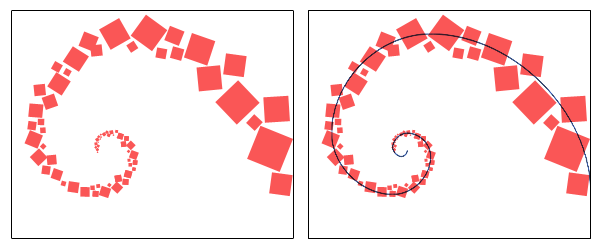
\includegraphics[scale=0.47]{graphics/fractal.png}
			\caption{Ejemplo de reconocimiento de una estructura fractal.}
			\label{fig:fractal}
			\end{figure}

		\item\textit{Ampliación de descripción del color de una figura:} la aplicación actual, con el objetivo de simplificar el proceso de análisis, sólo reconoce un color para cada figura reconocida. Sin embargo, hay multitud de formas que el ojo capta como una única mancha de color y aun así el color varía ligeramente dentro de la mancha en sí. Es por ello que puede ser de gran utilidad conseguir almacenar más información de color dentro de la representación de una figura.
	
	\end{itemize}
	
\item\textbf{Portar la aplicación a sistemas MACINTOSH.} Con esto se conseguiría expandir el número de posibles usuarios de la aplicación. Dado que las máquinas con sistema operativo de Apple funcionan con UNIX como base, esta ampliación puede resultar muy sencilla si se parte de la versión para Linux de la aplicación.

\item\textbf{Portar la aplicación a sistemas móviles.} Una de las ideas iniciales que se tuvieron en mente a la hora de realizar la aplicación fue la de implementar el sistema como una aplicación móvil. Sin embargo, al realizar un estudio del alcance del proyecto y el tiempo de desarrollo del mismo, se desechó la idea antes de comenzar el desarrollo. Sin embargo, una aplicación de esta índole puede alcanzar un gran éxito en estos dispositivos ya que las cámaras integradas de los mismos proporcionan una entrada gráfica fácil y sencilla, lo cual sumado a la facilidad de uso del sistema, dan a la aplicación un gran atractivo.\\

Teniendo esta ampliación en mente, el sistema se ha diseñado de forma que se facilite la portabilidad, eligiendo siempre librerías disponibles tanto en sistemas operativos de ordenadores personales como de dispositivos móviles (\todo{referenciar anexo de tecnologías}).\\

\end{itemize}

\todo{acabar con frase molona, que terminar con un itemize da palo}